\chapter{Analyse Aufgabenstellung}

Die Aufgabenstellung (siehe Anhang \ref{sec:aufgabenstellung}) verzichtet bewusst auf funktionale Anforderungen an die zu erstellende Applikation. Weiter werden auch keine spezifischen Technologien zur Umsetzung vorgegeben.

Diese sehr offene Ausgangssituation wird lediglich durch die folgenden Ansprüche eingegrenzt:

\begin{enumerate}
	\item Das Produkt soll unter Verwendung einer oder mehreren Internettechnologien konzipiert und umgesetzt werden.
	\item Der zu erstellende Quellcode soll \emph{State Of The Art} Architekturprinzipien \cite{ROCA} exemplarisch darstellen und der interessierten Fachperson als auch Studenten der Vorlesungs \emph{Internetnettechnologien} als Anschaungmaterial dienen können.
\end{enumerate}

Von diesen zwei Leitsätzen ausgehend kann angenommen werden, dass die Demonstration von Architekturprinzipien klar im Vordergrund stehen soll. Da diese Prinzipien aber auch einem lernenden Publikum (Punkt 2) so interessant wie möglich präsentiert werden sollen, ist eine attraktive Verpackung ebenfalls nicht zu vernachlässigen.

Dieses Kapitel beantwortet im weiteren Verlauf dementsprechend folgende Fragen genauer:

\begin{enumerate}
	\item Welche Schritte wurden im Bereich der Produkteentwicklung durchlaufen? Auf welche Aspekte wurde besonders eingegangen?
	\item Wie wurde die Technologie zur Umsetzung der generierten Produkteidee ausgewählt und welche Kriterien waren dabei ausschlaggebend?
\end{enumerate}

\section{Produktentwicklung}
Die Findung einer passenden Produktidee gestaltete sich unter den im vorherigen Abschnitt erwähnten Bedingungen nicht unbedingt als einfach:

Zwar soll ein Gros des Arbeitsaufwandes in das Entwickeln einer beispielhaften Architektur fliessen, diese soll aber in einem für Studierende möglichst attraktiven Gewand präsentiert werden.

\subsection{Workshop}
Um die zweitrangige Prozedur der Ideenfindung pragmatisch abhandeln zu können wurde ein Workshop mit Brainstorming und anschliessender Diskussionsrunde durchgeführt. Folgende Tabelle zeigt die Favoriten aus einem Pool generierter Ideen.

Die Spalte \emph{Potential} bewertet jede Idee nach subjektiver Einschätzung des Projektteams unter Berücksichtigung folgender Faktoren:
\begin{itemize}
	\item Funktionsumfang
	\item Konzeptionelle und technische Herausforderung
	\item Attraktivität (Für Projektteam)
	\item Attraktivität (Für Studierende des Moduls Internettechnologien)
\end{itemize}

\begin{table}[H]
\tablestyle
\tablealtcolored
\begin{tabularx}{\textwidth}{l X X c}
\tableheadcolor
	\tablehead Idee &
	\tablehead Pro &
	\tablehead Contra &
	\tablehead Potential \tabularnewline
\tablebody
	\textit{\gls{WG}-Aufgabenverwaltung} &
	Viele Studierende identifizieren sich tendenziell damit, da sie selber in einer \gls{WG} wohnen, Faktor \emph{Gamification} sehr interessant &
	&
	\faStar\faStar\faStar\tabularnewline

	\textit{Instant Messenger} &
	Attraktive Features wären realisierbar (Realtime, Websockets etc.) &
	Funktionelle Anforderungen könnten Rahmen sprengen &
	\faStar\faStar \tabularnewline

	\textit{Aufgabenverwaltung} &
	Evtl. gute Verwendung des Produkts &
	``\emph{Gibt's wie Sand am Meer}'', viele bestehende Beispielapplikationen \cite{TodoMVC} &
	\faStar\faStar \tabularnewline

	\textit{Chat} &
	&
	Bereits oft verwendet in bestehender Vorlesung, abgenutzte Thematik &
	\faStar \tabularnewline

	\textit{Forum} &
	&
	``\emph{Gibt's wie Sand am Meer}'' &
	\faStar \tabularnewline
\tableend
\end{tabularx}
\caption{Produktideenpool}
\end{table}

Am verheissungsvollsten wurde die Idee des \gls{WG} Aufgabenverwaltungstool eingeschätzt und gefiel dem gesamten Team von Beginn an ziemlich gut. Die Thematik \gls{Gamification} in einem konkreten Produkt umsetzen zu können eliminierte schlussendlich die letzten Zweifel.

In einem nächsten Schritt wurde die rohe Produktidee mit einem Mindmap (siehe Anhang \ref{sec:produktentwicklung}) weiter ausgebaut und die ersten funktionalen Anforderungen wurden entwickelt. Daneben konnte eine konkrete Kurzbeschreibung sowie das erste Branding für das geplante Produkt formuliert resp. entworfen werden.


\subsection{Die finale Produktidee: Roomies}
\emph{Roomies} soll einer \gls{WG} ermöglichen, anfallende Aufgaben leicht unter den verschiedenen Bewohnern zu organisieren. Damit auch langweilige Ämtchen endlich erledigt werden, schafft Roomies durch ein Ranglisten- und Badgesystem (\gls{Gamification}) einen Anreiz, um seine Mitbewohner übertrumpfen zu wollen.

Durch das Aufgreifen einer Thematik aus dem Studentenalltag soll Roomies für lernende aus dem Modul \emph{Internettechnologien} einen leichten Einstieg in die tendenziell trockene Materie der Softwarearchitektur bieten.

\subsection{Branding}
Der namensgebende Ausdruck \emph{Roomie} stammt aus dem US-amerikanischen und bedeutet soviel wie \emph{Mitbewohner} oder \emph{Zimmernachbar} \cite{Roomie}. Passend dazu soll neben dem Namen auch das restliche Produktbranding an die US-amerikanische College-Welt angelehnt werden.

Vom Logo über die Farbwahl bis zum späteren User Interface Design sollen folgende Stilelemente als roter Faden verwendet werden:

\begin{enumerate}
	\item \emph{Gedimmte} Farben, keine grellen Akzente
	\item Simple, aber eingängige und klar definierte Formensprache
	\item Serifen-betonte Schriftart als Stilmittel
\end{enumerate}

Im Folgenden sind die Grundlegenden Stilelemente zur Referenz aufgeführt. Das Produktlogo wird zudem in verschiedenen, grössenoptimierten Varianten gezeigt.

\subsubsection*{Grundfarbpalette}
\begin{figure}[H]
	\definecolor{spec_white}{HTML}{FFFFFF}
	\definecolor{spec_blue}{HTML}{1A3143}
	\definecolor{spec_red}{HTML}{A4000F}

	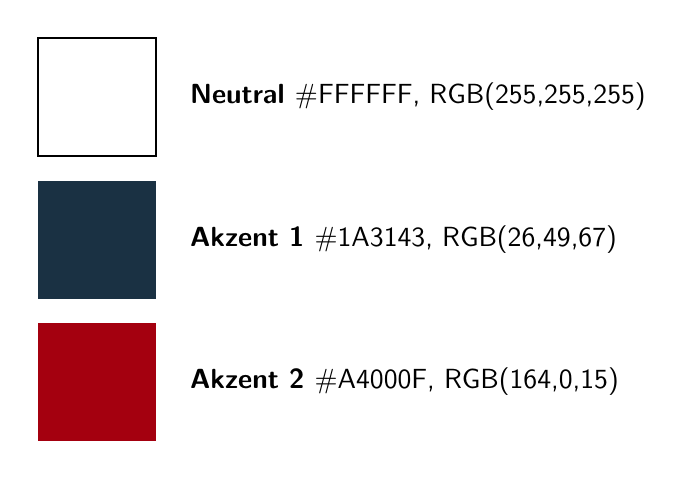
\begin{tikzpicture}
		\tikzstyle{colorswatch} = [rectangle,draw=none,minimum width=15mm,minimum height=15mm,thick];
		\tikzstyle{colorspec} = [draw=none,fill=none,right];

		\matrix[row sep=3mm, column sep=3mm]{
			\node[colorswatch,draw=black,fill=spec_white]{}; &
			\node[colorspec]{\sffamily\bfseries Neutral \normalfont\sffamily\#FFFFFF, RGB(255,255,255)}; \\
			\node[colorswatch,fill=spec_blue]{}; &
			\node[colorspec]{\sffamily\bfseries Akzent 1 \normalfont\sffamily\#1A3143, RGB(26,49,67)}; \\
			\node[colorswatch,fill=spec_red]{}; &
			\node[colorspec]{\sffamily\bfseries Akzent 2 \normalfont\sffamily\#A4000F, RGB(164,0,15)}; \\
		};
	\end{tikzpicture}
	\caption{Branding Farbpalette}
\end{figure}

\subsubsection*{Logo \& Logovariationen}
\begin{figure}[H]
	\centering
	
\includegraphics[width=5cm]{content/images/roomies-withshadow.png}
	\caption{Roomies Logo im College Stil}
\end{figure}

\begin{figure}[H]
	\centering
	
\includegraphics[width=10cm]{content/images/logo-variants.png}
	\caption{Roomies Logo in verschiedenen Grössen \& Varianten}
\end{figure}

\section{Technologieevaluation}
Das Thema ``Architekturkonzepte moderner Web-Applikationen'' legt den Schluss nahe, nicht nur aktuellste Architekturprinzipien bei der Umsetzung der Beispielapplikation zu verwenden, sondern auch im Bereich der Technologiewahl auf etablierte Platzhirsche wie Java oder C\# (in Verbindung mit deren Web-Frameworks) zu verzichten.

Unter Berücksichtigung der persönlichen Erfahrungen und Einschätzungen aller Projektteilnehmer wurde in Vereinbarung mit dem Betreuer im Zuge einer Evaluation eine Shortlist mit folgenden Technologiekandidaten zusammengestellt:

\begin{itemize}
	\item \emph{Ruby}\\
	Ruby hat sich in der näheren Vergangenheit zusammen mit Ruby On Rails im Markt etablieren können. Als relativ junge Technologie durfte es aus diesem Grund bei einer Evaluation nicht ignoriert werden.

	\item \emph{Java}\\
	Trotz des einführenden Statements, Platzhirsche von einer engeren Auswahl auszuschliessen, war das Projektteam aufgrund der vorangegangenen Studienarbeit davon überzeugt, dass Java, insbesondere als Backendtechnologie, mit den ``jungen Wilden'' problemlos mithalten kann.

	\item \emph{JavaScript}\\
	Während den letzten zwei Jahren erlebte JavaScript eine Renaissance: Mit node.js schaffte es den Sprung vom Frontend-Layer ins Backend und erfreut sich in der OpenSource als auch der Industrie-Community grösster Beliebtheit.
\end{itemize}

In diesem Abschnitt werden übergreifende Bewertungskriterien definiert, welche anschliessend auf alle drei Technologiekandidaten, resp. deren Frameworks angwendet werden können.

\newpage
\subsection{Bewertungskriterien \& Gesamtbewertung}
Die folgende Tabelle definert sechs Kriterien, welche zur Bewertung einer Technologie oder eines Frameworks jeweils mit 0-3 Sternen bewertet werden können.

Die Spalte \emph{Gewichtung} gibt an, als wie wichtig das betreffende Kriterium im Bezug auf die Aufgabenstellung anzusehen ist.

\begin{table}[H]
\tablestyle
\tablealtcolored
\begin{tabularx}{\textwidth}{l l X c}
\tableheadcolor
	\tablehead ID &
	\tablehead Kriterium &
	\tablehead Erläuterung &
	\tablehead Gewichtung \tabularnewline
\tablebody
\textit{TK1} &
	Eigenkonzepte &
	Wieviele eigene Konzepte \& Ideen bringt eine Technologie resp. ein Framework mit? Viele spezifische Konzepte bedeuten meistens eine steile Lernkurve für Neueinsteiger. \emph{Hohe Bewertung = Wenig Eigenkonzepte}&
	\faStar\faStar\faStar \tabularnewline
\textit{TK2} &
	Eignung &
	Wie gut eignet sich eine Technologie oder ein Framework für die Demonstration der Architekturrichtlinien? Geschieht alles ``hinter'' dem Vorhang oder sind einzelne Komponenten einsehbar? \emph{Hohe Bewertung = Hohe Eignung}&
	\faStar\faStar\faStar \tabularnewline
\textit{TK3} &
	Produktreife &
	Wie gut hat sich das Framework oder die Technologie bis jetzt in der Realität beweisen können? Wie lange existiert es schon? Gibt es eine aktive Community und wird es aktiv weiterentwickelt? \emph{Hohe Bewertung = Hohe Produktreife}&
	\faStar\faStar\faStar\tabularnewline
\textit{TK4} &
	Aktualität &
	Diese Arbeit kümmert sich um ``moderne Web-Applikationen''. So sollte auch die zu verwendende Technologie gewissermassen nicht von ``vorgestern'' sein. \emph{Hohe Bewertung = Hohe Aktualität}&
	\faStar \tabularnewline
\textit{TK5} &
	``Ease of use'' &
	Wie angenehm ist das initiale Erstellen, die Konfiguration und die Unterhaltung einer Applikation? Führt das Framework irgendwelchen ``syntactic sugar'' \cite{syntacticsugar} ein um die Arbeit zu erleichtern? \emph{Hohe Bewertung = Hoher ``Ease of use''-Faktor} &
	\faStar\faStar \tabularnewline
\textit{TK6} &
	Testbarkeit &
	Wie gut können die mit dem Framework oder der Technologie erstellte Komponenten durch Unit Tests getestet werden? \emph{Hohe Bewertung = Hohe Testbarkeit} &
	\faStar\faStar \tabularnewline
\tableend
\end{tabularx}
\caption{Bewertungskriterien für Technologieevaluation}
\label{tab:bewertungskriterien}
\end{table}


Für jedes Framework wird abschliessend eine Gesamtbewertung in Form einer Zahl errechnet. Dies geschieht mit folgender Formel:

\begin{figure}[H]
	\centering
	\large
	\begin{math}
		\frac{\sum \limits_{n=1}^6 Bewertung_{TK_n} \times {Gewichtung_{TK_n}}}{6}
	\end{math}
	\caption{Berechnungsformel Gesamtbewertung}
\end{figure}


\newpage
\subsection{Ruby}

Insbesondere mit dem Framework \emph{Ruby on Rails} \cite{RubyOnRails} wurde Ruby für die Entwicklung von Umfangreichen Webapplikationen seit Veröffentlichung in den 90ern immer beliebter. Mit fast kindlicher Selbstverständlichkeit bringt Ruby viele Konzepte wie \gls{Multiple Inheritance} (in Form von Mixins) oder die funktionale Behandlung von jeglichen Werten/Objekten von Haus aus mit.

Für den Einsteiger etwas verwirrend setzt es zudem auf eine für den Menschen ``leserlichere'' Syntax als beispielsweise von Java oder anderen verwandten Sprachen gewohnt. Folgende Codebeispiele bewirken die selbe Ausgabe auf der Kommandozeile, unterscheiden sich aber deutlich in ihrer Formulierung:

\begin{lstlisting}[language=Java, caption=Negierte if-Abfrage in Java]
if(!enabled) {
	System.out.println("Ich bin deaktiviert!");
}
\end{lstlisting}

\begin{lstlisting}[language=Ruby, caption=Negierte if-Abfrage in Ruby]
puts "Ich bin deaktiviert!" unless enabled
\end{lstlisting}

Während der kurzen Technologieevaluationsphase wurde im Bereich Ruby das Hauptaugenmerk auf \emph{Ruby on Rails} gelegt. Insbesondere die \gls{Scaffolding}tools und der daraus generierte Quellcode wurde näher begutachtet. Die Resultate sind wiederum auf die sechs Bewertungskriterien appliziert worden.

\subsubsection*{Bewertung Ruby on Rails}
\begin{table}[H]
\newcolumntype{s}{>{\centering\hsize=0.15\hsize}X}
\tablestyle
\tablealtcolored
\begin{tabularx}{\textwidth}{X s s s s s s s}
\tableheadcolor
	\tablehead &
	\rotatebox{90}{\bfseries\textit{TK1 Eigenkonzepte} } &
	\rotatebox{90}{\bfseries\textit{TK2 Eignung}} &
	\rotatebox{90}{\bfseries\textit{TK3 Produktreife}} &
	\rotatebox{90}{\bfseries\textit{TK4 Aktualität}} &
	\rotatebox{90}{\bfseries\textit{TK5 ``Ease of use''}} &
	\rotatebox{90}{\bfseries\textit{TK6 Testbarkeit}} &
	\rotatebox{90}{\bfseries\textit{Gesamtbewertung}}
	\tabularnewline
\tablebody
	\textit{Ruby on Rails} &
	\oneStar &
	\oneStar &
	\threeStars &
	\oneStar &
	\threeStars &
	\twoStars &
	\directlua{
		tex.print(math.round(
			(1 * 3 +
			1 * 3 +
			3 * 3 +
			1 * 1 +
			3 * 2 +
			2 * 2) / 6
		))
	}
	\tabularnewline
\tableend
\end{tabularx}
\caption{Bewertung Ruby on Rails}
\end{table}


\subsubsection*{Interpretation}
Nach genauerem Befassen mit Ruby on Rails sind die Einschätzung des Projektteams gespalten.

Zum Einen minimiert Ruby on Rails den Aufwand für das Erledigen von Routineaufgaben extrem (\gls{Scaffolding}). Der generierte Code ist sofort verwendbar und, gute Ruby-Kenntnisse vorausgesetzt, gut erweiterbar.

Zum Anderen ist aber gerade die Einfachheit, wie bspw. Controllers oder Models erzeugt und in den Applikationsablauf eingebunden werden, alles Andere als optimal wenn es darum geht, Architekturrichtlinien eindeutig und klar demonstrieren zu können.

Unter dem Vorbehalt, dass Ruby on Rails für die Demonstration der definierten Architekturrichtlinien evtl. nicht die richtige Wahl sein könnte, kann das Projektteam nur eine bedingte Empfehlung für das Ruby Framework abgeben.

\subsection{Java}

Schon vor dieser Bachelorarbeit kann das Projektteam diverse Erfahrungen mit Java vorweisen. Zum Einen aus privaten und beruflichen Projekten, zum Anderen auch ganz themenspezifisch aus der Studienarbeit, welche ein Semester früher durchgeführt wurde.

Als Teil einer grösseren Applikation wurde dort ein Webservice mit REST-Schnittstelle umgesetzt. Zum Einsatz kamen diverse Referenzimplementierungen von Java Standard API's. Die sehr positiven Erfahrungen mit der dort orchestrierten Zusammenstellung von Bibliotheken legen den Schluss nahe, diese auch für eine potentielle Verwendung innerhalb dieser Bachelorarbeit wiederzuverwenden.

Der Studienarbeit-erprobten Kombination sollen jedoch auch andere Alternativen gegenübergestellt werden. Insgesamt ergeben sich so folgende Analysekandidaten im Bereich der Technologie \emph{Java}:

\begin{table}[H]
\tablestyle
\tablealtcolored
\begin{tabularx}{\textwidth}{l X l}
\tableheadcolor
	\tablehead Framework &
	\tablehead Erläuterung \tabularnewline
\tablebody
\textit{Studienarbeit-Zusammenstellung} &
	Die Zusammenstellung von \emph{Google Guice}, \emph{Jersey}, \emph{Codehaus Jackson} sowie \emph{EclipseLink} hat sehr gut harmoniert. Die Verwendung von einem Java-fremden Framework für die Implementierung des Frontends wäre jedoch erneut abzuklären.
	\tabularnewline
\textit{Spring} &
	Spring hat sich in den letzten Jahren in der Industrie etablieren können. Es bietet eine Vielzahl von Subkomponenten (MVC, Beanmapping etc.).
	\tabularnewline
\textit{Plain JEE} &
	Java Enterprise bietet von sich aus viele Features, welche die Frameworks von Dritten unter anderen Ansätzen umsetzen. Es gilt jedoch abzuwägen, wie gross der Aufwand ist, um beispielsweise eine REST-Serviceschnittstelle zu implementieren.
	\tabularnewline
\textit{Vaadin} &
	Vaadin baut auf Googles GWT und erlaubt die serverlastige Entwicklung von Webapplikationen.
	\tabularnewline
\textit{Play! Framework} &
	Seit dem Release der Version 2.0 im Frühjar 2012 erfreut sich das Play! Frameworks grosser Beliebtheit. Insbesondere die integrierten Scaffolding-Funktionalitäten und MVC-Ansätze werden gelobt.
	\tabularnewline
\tableend
\end{tabularx}
\caption{Shortlist Analysekandidaten Java}
\end{table}


\subsubsection*{Bewertungsmatrix}

\begin{table}[H]
\newcolumntype{s}{>{\centering\hsize=0.15\hsize}X}
\tablestyle
\tablealtcolored
\begin{tabularx}{\textwidth}{X s s s s s s s}

\tableheadcolor
	\tablehead &
	\rotatebox{90}{\bfseries\textit{TK1 Eigenkonzepte} } &
	\rotatebox{90}{\bfseries\textit{TK2 Eignung}} &
	\rotatebox{90}{\bfseries\textit{TK3 Produktreife}} &
	\rotatebox{90}{\bfseries\textit{TK4 Aktualität}} &
	\rotatebox{90}{\bfseries\textit{TK5 ``Ease of use''}} &
	\rotatebox{90}{\bfseries\textit{TK6 Testbarkeit}} &
	\rotatebox{90}{\bfseries\textit{Total}}
	\tabularnewline
\tablebody
	\textit{Studienarbeit-Zusammenstellung}	&
	\threeStars &
	\threeStars &
		&
		&
	\threeStars &
	\twoStars &
	\directlua{
		tex.print(math.round(
			(3 * 3 +
			3 * 3 +
			0 * 3 +
			0 * 1 +
			3 * 2 +
			2 * 1) / 6
		))
	}
	\tabularnewline


	\textit{Spring} &
		&
		&
	\twoStars &
	\threeStars &
		&
	\oneStar &
	\directlua{
		tex.print(math.round(
			(0 * 3 +
			0 * 3 +
			2 * 3 +
			3 * 1 +
			0 * 2 +
			1 * 1) / 6
		))
	}
	\tabularnewline


	\textit{Plain JEE} &
		&
	\twoStars &
	\threeStars &
	\threeStars &
		&
	\threeStars &
	\directlua{
		tex.print(math.round(
			(0 * 3 +
			2 * 3 +
			3 * 3 +
			3 * 1 +
			0 * 2 +
			3 * 1) / 6
		))
	}
	\tabularnewline


	\textit{Vaadin} &
	\oneStar &
		&
	\threeStars &
	\twoStars &
		&
	\threeStars &
	\directlua{
		tex.print(math.round(
			(1 * 3 +
			0 * 3 +
			3 * 3 +
			2 * 1 +
			0 * 2 +
			3 * 1) / 6
		))
	}
	\tabularnewline


	\textit{Play! Framework} &
	\oneStar &
	&
	\twoStars &
	\twoStars &
	&
	\threeStars&
	\directlua{
		tex.print(math.round(
			(1 * 3 +
			0 * 3 +
			2 * 3 +
			2 * 1 +
			0 * 2 +
			3 * 1) / 6
		))
	}
	\tabularnewline
\tableend
\end{tabularx}
\caption{Bewertungsmatrix Java Frameworks}
\end{table}

\subsubsection*{Interpretation}
\emph{Plain JEE}, \emph{Vaadin} und \emph{Play! Framework} spielen ihre Stärken klar in der Produktreife und der dadurch hohen Wartbarkeit resp. Testbarkeit aus. Im Bezug auf die Eigenkonzepte benötigen alle Kandidaten einen gewissen initialen Lernaufwand. \emph{Studienarbeit-Zusammenstellung} arbeitet mit einem klar zugänglichen Schichtenmodell und verwendet über dies hinaus ein komplett vom Backend entkoppeltes Frontend. Zwar wäre eine solche Lösung auch mit \emph{Spring} und \emph{Plain JEE} möglich, jedoch versagen diese beiden Frameworks wiederum im Bezug auf die Eignung, die aufgestellten Architekturrichtlinien transparent demonstrieren zu können.

Die Produktreife von \emph{Studienarbeit-Zusammenstellung} ist zu vernachlässigen. Die einzelnen Komponenten für sich haben sich bereits in länger in der Praxis bewähren können und sind lediglich genau in dieser Kombination evtl. weniger oft erprobt.

Für die endgültige Auswahl einer Technologie schickt Java aufgrund vorangegangener Bewertung die \emph{Studienarbeit-Zusammenstellung} in die finale Ausscheidung.

\subsection{JavaScript}
\label{sec:technology-evaluation-javascript}

JavaScript ist insbesondere als ``Webprogrammiersprache'' bekannt. In den vergangenen Jahren wurde es hauptsächlich innerhalb des Internetbrowsers verwendet, um starre Internetseiten mit mehr Interaktivität zu versehen. Insbesondere die Anstrengungen von Mozilla \cite{SpiderMonkey} und Google \cite{V8JavaScript} verhalfen der früher für schlechte Performance und schlechte Codequalität verschrieenen Programmiersprache zu neuem Glanz.

Mit JavaScript sind heute innerhalb des Browsers komplexe und umfangreiche Applikationen problemlos umzusetzen und weit verbreitet.

Die quelloffene V8 JavaScript Engine \cite{V8JavaScript} von Google hat 2009 zudem den Sprung weg vom Browser geschafft: node.js \cite{nodejs} bietet die Engine als eigenständigen Skriptinterpreter an und verfügt über eine umfangreiche, leistungsstarke und systemnahe API. Die neu entstandene Plattform erfreut sich in der Opensource Community grösster Beliebtheit. So sind seit der ersten Veröffentlichung eine Vielzahl an Frameworks und Bibliotheken zu den verschiedensten Themengebieten entstanden.

Auch im Bereich der Webframeworks gibt es auf diese Weise eine Menge an interessanten Libraries zu entdecken. Für die Evaluation im Bezug auf diese Bachelorarbeit werden folgende Frameworks genauer analysiert:

\begin{table}[H]
\tablestyle
\tablealtcolored
\begin{tabularx}{\textwidth}{l X l}
\tableheadcolor
	\tablehead Framework &
	\tablehead Erläuterung \tabularnewline
\tablebody
\textit{Express.js} &
	Express.js \cite{Expressjs} baut auf dem Basisframework Connect \cite{connect} auf. Das damit durchgängig umgesetzte Middleware-Konzept ermöglicht die entkoppelte Entwicklung von simplen Webservern bis hin ausgefeilten Webservices. Zu Beginn genügen max. 10 Zeilen Quellcode, um einen GET-Request \cite{HTTPRequest} entgegen zu nehmen und eine Antwort an den Aufrufer zurück zu senden. Dem Ausbau zu komplexeren Applikationen steht dank der erwähnten Middleware-Architektur jedoch nichts im Wege.
	\tabularnewline
\textit{Tower.js} &
	Pate für Tower.js \cite{towerjs} steht nach eigenen Angaben des Entwicklers Ruby on Rails. Entsprechend umfangreich sind auch hier die \gls{Scaffolding}funktionalitäten. Das Framework selbst ist mit CoffeeScript \cite{CoffeeScript} entwickelt worden. Wie das Ruby-Vorbild bietet auch Tower.js ein ausgewachsenes MVC-Pattern zur Entwicklung eigener Applikationen an.
	\tabularnewline
\textit{derby} &
	Das Framework Derby \cite{Derby} nimmt sich das oben eingeführte Express.js zur Grundlage und erweitert es im das Model-View-Controller-Pattern. Es bleibt dabei extrem leichtgewichtig, ermöglicht aber leider keine Browserclients welche der Anforderung des \emph{Unobtrusive JavaScripts} genügen mögen: Derby-Applikationen werden komplett im Browser gerendert und bieten keine Möglichkeit, HTML-Markup auf dem Server zu generieren.
	\tabularnewline
\textit{Geddy} &
	Mit Geddy \cite{Geddy} begibt sich bereits der zweite Kandidat für node.js in den Ring, welcher sich Ruby on Rails zum Vorbild nimmt. Dementsprechend vergleichbar ist der Funktionsumfang mit Tower.js. Als wichtiger Unterschied ist jedoch zu erwähnen, dass Geddy auf CoffeeScript vollends verzichtet.
	\tabularnewline
\textit{Sails} &
	Sails \cite{sails} ist der jüngste Frameworkkandidat für JavaScript resp. node.js. Die Grundkonzepte von Ruby on Rails werden mit einer Prise ``Realtime'' (\glspl{Websocket}) gewürzt. So kann jede Ressource über eine einfache REST-Schnittstelle als auch über eine Websocket-Verbindung angesprochen werden. Damit erleichtert sich das asynchrone resp. servergesteuerte Aktualisieren des Frontends.
	\tabularnewline
\tableend
\end{tabularx}
\caption{Shortlist Analysekandidaten JavaScript}
\end{table}



\subsubsection*{Bewertungsmatrix}

\begin{table}[H]
\newcolumntype{s}{>{\centering\hsize=0.15\hsize}X}
\tablestyle
\tablealtcolored
\begin{tabularx}{\textwidth}{X s s s s s s s}
\tableheadcolor
	\tablehead &
	\rotatebox{90}{\bfseries\textit{TK1 Eigenkonzepte} } &
	\rotatebox{90}{\bfseries\textit{TK2 Eignung}} &
	\rotatebox{90}{\bfseries\textit{TK3 Produktreife}} &
	\rotatebox{90}{\bfseries\textit{TK4 Aktualität}} &
	\rotatebox{90}{\bfseries\textit{TK5 ``Ease of use''}} &
	\rotatebox{90}{\bfseries\textit{TK6 Testbarkeit}} &
	\rotatebox{90}{\bfseries\textit{Total}}
	\tabularnewline
\tablebody
	\textit{Express.js}	&
	\threeStars &
	\threeStars	&
	\twoStars &
	\threeStars &
	\twoStars &
	\threeStars &
	\directlua{
		tex.print(math.round(
			(3 * 3 +
			3 * 3 +
			2 * 3 +
			3 * 1 +
			2 * 2 +
			3 * 2) / 6
		))
	}
	\tabularnewline

	\textit{Tower.js} &
	\twoStars &
	\twoStars &
	\oneStar &
	\threeStars &
	\threeStars	&
		&
	\directlua{
		tex.print(math.round(
			(2 * 3 +
			2 * 3 +
			1 * 3 +
			3 * 1 +
			3 * 2 +
			0 * 2) / 6
		))
	}
	\tabularnewline


	\textit{derby} &
	\twoStars &
	\oneStar &
	\oneStar &
	\threeStars &
	\twoStars &
		&
	\directlua{
		tex.print(math.round(
			(2 * 3 +
			1 * 3 +
			1 * 3 +
			3 * 1 +
			2 * 2 +
			0 * 2) / 6
		))
	}
	\tabularnewline


	\textit{Geddy} &
	\threeStars &
	\oneStar &
	\twoStars &
	\twoStars &
	\threeStars &
	&
	\directlua{
		tex.print(math.round(
			(3 * 3 +
			1 * 3 +
			2 * 3 +
			2 * 1 +
			3 * 2 +
			0 * 2) / 6
		))
	}
	\tabularnewline


	\textit{Sails} &
	\twoStars &
	\twoStars &
	\oneStar &
	\threeStars &
	\twoStars &
	\oneStar &
	\directlua{
		tex.print(math.round(
			(2 * 3 +
			2 * 3 +
			1 * 3 +
			3 * 1 +
			2 * 2 +
			1 * 2) / 6
		))
	}
	\tabularnewline
\tableend
\end{tabularx}
\caption{Bewertungsmatrix JavaScript Frameworks}
\end{table}

